\documentclass[12pt, a4paper]{article}
    
\usepackage{homework}
\usepackage{amsmath}				% For Math
\usepackage{graphicx}				% For including figure/image
\usepackage{cancel}					% To use the slash to cancel out stuff in work
\usepackage{multirow}
\usepackage{lastpage}
\usepackage{pdfpages}

\usepackage[
backend=biber,
% style=alphabetic,
sorting=ynt,
date=iso,
urldate=iso
]{biblatex}
\addbibresource{refs.bib}

\usepackage[firstpage=true]{background}
\backgroundsetup{
    scale=0.3,
    angle=0,
    opacity=0.1,
    contents={%
        \includegraphics[scale=1]{figs/Emblem_of_CU.png}
    }
}

%%%%%%%%%%%%%%%%%%%%%%
% Set up fancy header/footer
\pagestyle{fancy}
\setlength{\headheight}{28pt}
\fancyhead[LO,L]{CENG3430 Rapid Prototyping of Digital System\\Author: C.H. Yu, C.H. Sennett Cheng}
\fancyhead[CO,C]{}
\fancyhead[RO,R]{Final Project\\Date: \today}
\fancyfoot[LO,L]{}
\fancyfoot[CO,C]{}
% \fancyfoot[RO,R]{Page \thepage\ of \pageref{LastPage}}
\renewcommand{\headrulewidth}{0.4pt}
\renewcommand{\footrulewidth}{0.4pt}

\setcounter{secnumdepth}{3}
\setcounter{tocdepth}{3}
%%%%%%%%%%%%%%%%%%%%%%

\begin{document}  

\begin{titlepage}
    \begin{center}

		\bf\LARGE{The Chinese University of Hong Kong}
        \bf\Large{Department of Computer Science\\and Engineering}
		
		\vspace{80pt}
		
		\vspace{15pt}
		\textbf{\Large CENG3430 Rapid Prototyping of Digital System\\}
		\vspace{10pt}
		\textbf{\Large Final Project - FPGA-based Computer Vision Accelerator for Train Active Safety System}\\
		\vspace{10pt}
		\textbf{\Large Report}\\
        \vspace{6pt}
        % {\large Project Demo Date: 16 May 2025}\\
        {\large Project Demo Deadline: 16 May 2025 23:59}
		\vspace{40pt}
		
        \vspace{15pt}
		\textbf{\normalsize
            1155193237 - Yu Ching Hei (chyu2@cse.cuhk.edu.hk)\\
            1155206044 - Cheng Chung Hei Sennett(1155206044@link.cuhk.edu.hk)\\
        }
		\vspace{40pt}
        \textbf{\large Source code and project history is available on GitHub:}\\
        \normalsize \url{https://github.com/Jellyfish227/FPGA_Accelerated_Computer_Vision_on_Train_Active_Safety_System.git}\\
        \vspace{60pt}
		\textit{Under the kind support and guidance of}\\
		\textbf{\large Prof. Ming-Chang YANG}\\
		\vspace{20pt}
        % \textit{Also thank you for the help provided by teaching assistants}\\
		% \textbf{\large 
        %     Mr. Kezhi LI\\
        %     Mr. Han ZHAO\\
        %     Mr. Zhirui ZHANG\\
        % }
		
	\end{center}
\end{titlepage}

\pagenumbering{roman}
\setcounter{page}{2}
\fancyfoot[RO,R]{Page \thepage}

\tableofcontents

\section*{Division of Work}
\begin{tabularx}{\textwidth}{|l||X|}
    \hline
    \textbf{Task} & \textbf{Person In Charge} \\
    \hline\hline
    \textbf{Project Proposal} & Cheng Chung Hei Sennett \\
    \hline
    \textbf{Data Pre-processing} & Yu Ching Hei, Cheng Chung Hei Sennett \\
    \hline
    \textbf{AI-Inferencing} & Yu Ching Hei \\
    \hline
    \textbf{Post-processing} & Cheng Chung Hei Sennett \\
    \hline
    \textbf{Report} & Yu Ching Hei \\
    \hline
\end{tabularx}

\newpage
\pagenumbering{arabic}
\setcounter{page}{1}
\fancyfoot[RO,R]{Page \thepage\ of \pageref{LastPage}}

\section{Introduction}
% What is the system you want to design? Why?
% detailed account of the project objectives
% and achievements (for future reference, evaluation, and even
% reproduction)

The CENG3430 final project involved implementing a computer vision acceleration platform on the Zynq UltraScale+ MPSoC \cite{zynq_ultrascale_swdev}
that can be used to implement a train active safety system.

\noindent The workflow consists of two phases:
\begin{enumerate}
    \item \textbf{Data Pre-processing:} We collect and process the data from the camera from PS USB port, then port the video stream to the PL DPU. 
    \item \textbf{Data AI-Inferencing:} The DPU contains a set of pre-trained models that will perform lane detection, object detection, depth-of-field estimation and drivable area prediction.
    \item \textbf{Data Post-processing:} The PS should release PWM signals to control the motors to stop the rotation. But in our actual implementation, we don't really have enough time to implement the remaining actuators. 
\end{enumerate}
This report outlines our challenges faced and insights gained during implementation, aiming to deliver a fast and efficient computer vision acceleration platform for train active safety system.

\section{Design flow}
Overview: Describe the overall architecture, inputs, and outputs of the
system.
You are highly suggested to use flowcharts and block diagrams for
better presentation.
Module Descriptions: Discuss each module of the system clearly and
the interactions among them.

\subsection{Choice of board}
We have decided to use the Zynq UltraScale+ MPSoC ZCU102 and ZCU104 \cite{zynq_ultrascale_swdev} as our development board instead of 
using the original ZedBoard \cite{zedboard_docs} as the original ZedBoard is not supported by the Vitis AI library.

The Zynq UltraScale+ platform provides the following features:
\begin{itemize}
    \item More logic resources
    \item More powerful processing unit, including the Real-Time Processing Unit (RPU)
    \item More support for AI, including the Vitis AI library
\end{itemize}

\subsection{Phase 1: Data Pre-processing}
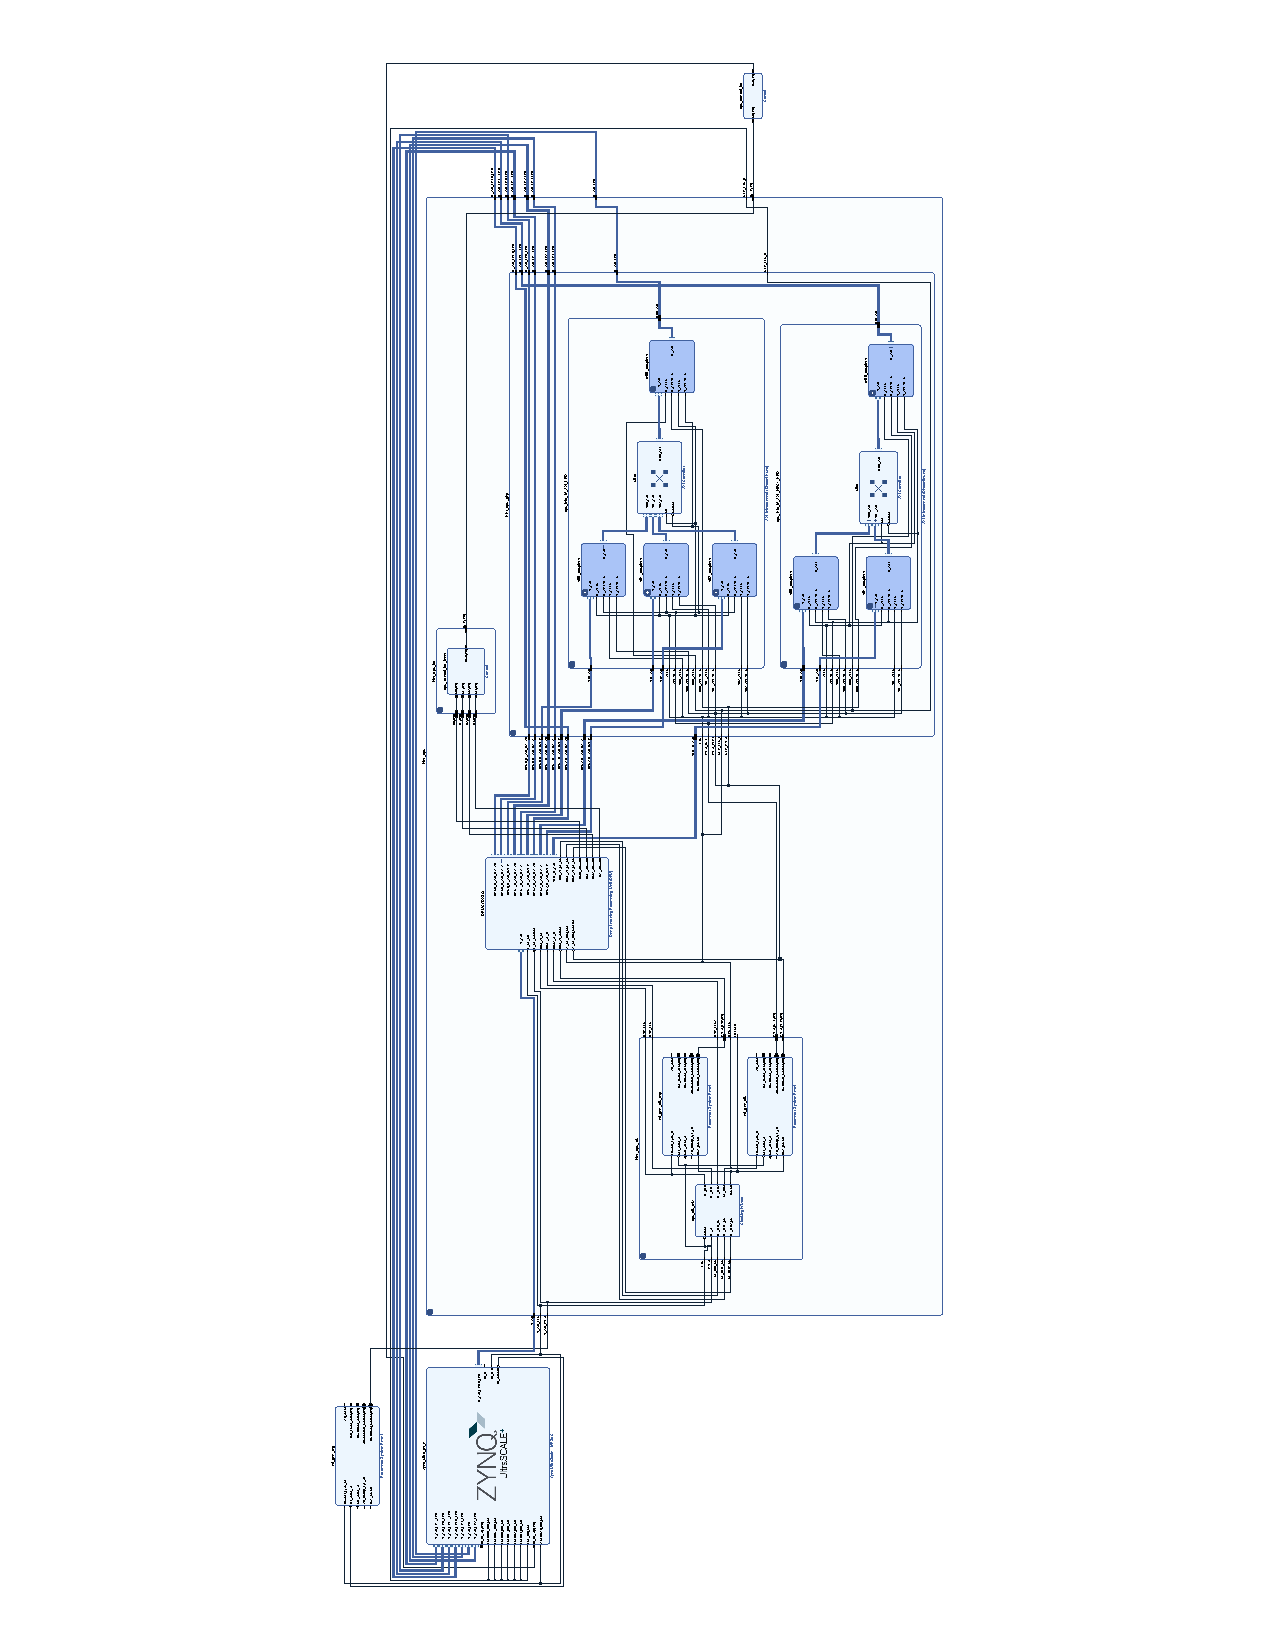
\includepdf[pages=-]{figs/DPUBlockDesign.pdf}
In this stage, in order to prototype the input in the most efficient way, we make use of the given USB protocal from the PS side. 
We have tried to utilize the RPU to do the continues video fetch, but we were not able to find a way to achieve this, so we just use the normal approach that fetch the video fram from the USB port, 
then pass the frame to the DPU with the AXI HP inteconnect. Which allows bandwidth up to 128bits. 


\subsection{Phase 2: Data AI-Inferencing}
This is the main part of this project. Unfortunatly, due to the time constraint, we were not able to implement a dataflow-based accelerator implementation. 
Therefore, we decided to leverage the Vitis AI library together with the soft DPU IP to implement the accelerator and deploying the pre-trained models. 

\subsection{Phase 3: Data Post-processing}


\section{Implementation}
Discuss in detail how you implement the system, you can take
screenshots to provide step-by-step instructions, or explain the source
code(s) part by part. You can also provide the screenshot of the
validated block design (if any).

\section{Results}
What have you achieved? Have you realized the preset goals?
What are the difficulties or limitations encountered during the
implementation, and how you resolved them?
What are the further improvement and possibilities?

\section{Conclusion}
To sum up, we have successfully implemented a responsive laser turret that can capture the motion of hand and reflect it to the laser turret wirelessly.
\newline
Before working on this project, we have expected that the most challenging part would be the motion capturing part. 
But surprisingly, we found that the most challenging part was actually the data transmission part, which we have to ensure the data integrity and stability.
Through this iterative process of design, implementation, and debugging, we have gained valuable insights into embedded systems development. 
These experiences and lessons learned will prove invaluable for future embedded systems projects encountered.

\section{References}
\printbibliography[heading=none]

\end{document}